\begin{figure}
	
	\ifdraft{}{
		\begin{subfigure}[t]{0.34\textwidth}
			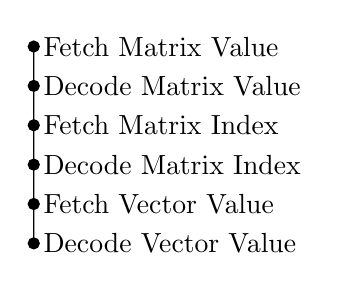
\begin{tikzpicture}
				\filldraw
					(0,2.5) circle (2pt) node[right] {Fetch Matrix Value} --
					(0,2.0) circle (2pt) node[right] {Decode Matrix Value} --
					(0,1.5) circle (2pt) node[right] {Fetch Matrix Index} --
					(0,1.0) circle (2pt) node[right] {Decode Matrix Index} --
					(0,0.5) circle (2pt) node[right] {Fetch Vector Value} --
					(0,0.0) circle (2pt) node[right] {Decode Vector Value};
			\end{tikzpicture}
			\caption{Serial Model.}
		\end{subfigure}
		\begin{subfigure}[t]{0.65\textwidth}
			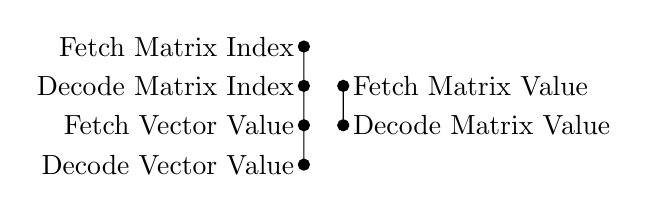
\begin{tikzpicture}
				\filldraw
					(0,2.0) circle (2pt) node[left] {Fetch Matrix Index} --
					(0,1.5) circle (2pt) node[left] {Decode Matrix Index} --
					(0,1.0) circle (2pt) node[left] {Fetch Vector Value} --
					(0,0.5) circle (2pt) node[left] {Decode Vector Value};
				\filldraw
					(0.5,1.5) circle (2pt) node[right] {Fetch Matrix Value} --
					(0.5,1.0) circle (2pt) node[right] {Decode Matrix Value};
			\end{tikzpicture}
			\caption{Parallel Model.}
		\end{subfigure}
	}
	
	\caption[Data dependency graphs for performance models.]{Comparison of the data dependency graphs used by each model, where lower nodes are dependent on higher nodes.}
	\label{fig:models-dataDeps}
\end{figure}